\documentclass[a4paper, 11pt]{article}
\usepackage[utf8]{inputenc}
\usepackage{graphicx,wrapfig,subfigure,amsmath,amssymb,epsfig,bm}
\usepackage{listings,textcomp,color,geometry,siunitx}
\usepackage{hyperref}
\geometry{hmargin=2cm, vmargin=2cm}


\def\Box{\mathord{\dalemb{7.9}{8}\hbox{\hskip1pt}}}
\def\dalemb#1#2{{\vbox{\hrule height.#2pt
        \hbox{\vrule width.#2pt height#1pt \kern#1pt \vrule width.#2pt}
        \hrule height.#2pt}}}

\def\eop{\mathcal{E}}
\def\bop{\mathcal{B}}
\def\ba{\begin{eqnarray}}
\def\ea{\end{eqnarray}}
\def\be{\begin{equation}}
\def\ee{\end{equation}}
\def\tr{{\rm tr}}
\def\Var{{\rm Var}}
\def\gtorder{\mathrel{\raise.3ex\hbox{$>$}\mkern-14mu
             \lower0.6ex\hbox{$\sim$}}}
\def\ltorder{\mathrel{\raise.3ex\hbox{$<$}\mkern-14mu
             \lower0.6ex\hbox{$\sim$}}}

\def\bb{{\mathfrak b}}
\newcommand{\ellb }{\boldsymbol{\ell }}

% Personal colors defined here
\newcommand{\skn}[1]{{\color{red}#1}}
\newcommand{\TIB}[1]{{\color{blue}#1}}
\newcommand{\assume}[1]{{\bf#1}}

\begin{document}

\title{\textbf{Scientific Documentation: maps2params}}
\maketitle

This document serves as a draft for the documentation of the maps2params pipeline. The goal is to clarify what exactly goes into the simulations and to report on the current results we are getting. The document is expected to evolve with time when more and more complexity is added to the pipeline.
We are currently set up to generate and analyse simplistic simulations of the SO large aperture telescope and of the Planck satellite.

\section{Generation of simulations}

\subsection{Sky model}

We model the sky as the sum of CMB fluctuations and extra galactic foregrounds, specifically we use the Dunkley et al sky model
\ba
T^{\nu}(\hat{n}) &=&  T^{\rm CMB}(\hat{n}) + T^{\nu, \rm tSZ}(\hat{n}) + T^{\nu, \rm kSZ}(\hat{n}) + T^{\nu, \rm CIB-P}(\hat{n}) + T^{\nu, \rm CIB-C}(\hat{n}) + T^{\nu, \rm rad}(\hat{n}) \nonumber \\
Q^{\nu}(\hat{n}) &=& Q(\hat{n}) \nonumber \\
U^{\nu}(\hat{n}) &=& U(\hat{n})
\ea
Note that we did not include foreground in polarisation and that we did not include galactic foregrounds yet. For these simplistic simulations, we furthermore assume that the entire sky follow a gaussian distribution and can therefore be entirely described by the power spectra
\ba
C^{\nu_{1} \nu_{2}}_{\ell} = C^{\rm CMB}_{\ell} + C^{ \rm kSZ}_{\ell}   + C^{\nu_{1} \nu_{2}, \rm tSZ}_{\ell}  + C^{\nu_{1} \nu_{2}, \rm CIB-P}_{\ell} + C^{\nu_{1} \nu_{2}, \rm CIB-C}_{\ell} + C^{\nu_{1} \nu_{2}, \rm rad}_{\ell}
\ea
Note that for now, we are neglecting cross correlation between different components, in particular the CIB-tSZ correlation. The extra-galactic components are generated using the fgspectra and we use a set of amplitude consistent with Dunkley et al (therefore consistent with the ACT 15 mJy source flux cut)
We display the foreground model for two frequencies (145 and 225 GHz) in Figure \ref{fig:fg_model}. Note that bandpasses integration is not yet implemented so bandpasses are assumed to be Dirac functions. 

\begin{figure*}
  \centering
  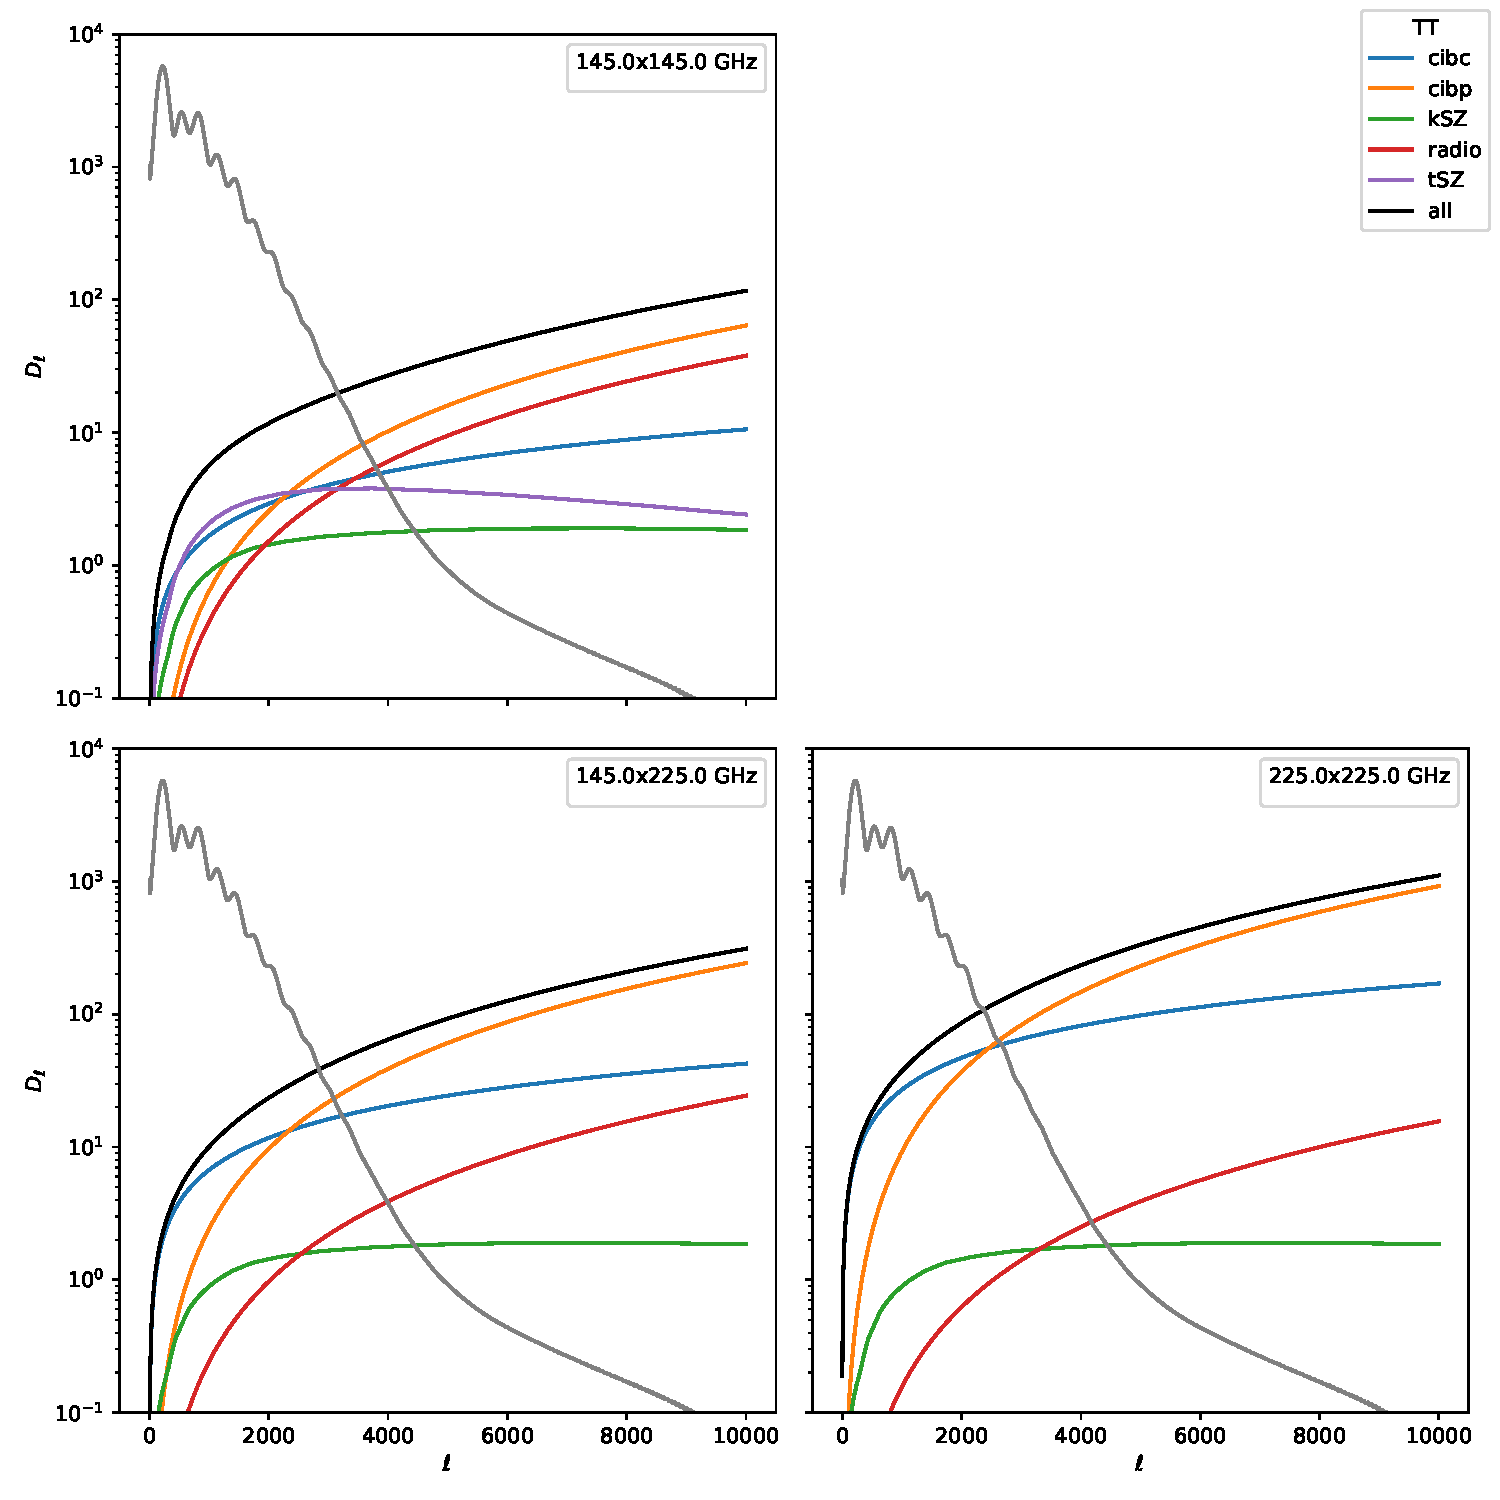
\includegraphics[width=1 \textwidth]{foregrounds.pdf}
  \caption{Foreground model for the the maps2params project.}
  \label{fig:fg_model}
\end{figure*}

\subsection{Noise model}

The large aperture telescope noise is modelled as a white noise component plus an atmospheric  component
\ba
N_{\ell} = N^{\rm white}_{\ell} + N^{\rm red}_{\ell}
\ea
The specifications for noise amplitude are the ones of the so noise calculator (specifically the version ${\it so\_noise\_calculator\_public\_20180822}$) which we believe is slighty outdated. The planck noise is modelled as white with specifications given by Table 4 of https://arxiv.org/pdf/1807.06205.pdf.
We display the noise model in Figure \ref{fig:noise_model}. Note that we display the effective noise power spectra, that is,  noise power spectra divided by the beam window functions. The current simulations assume homogeneous noise.

\begin{figure*}
  \centering
  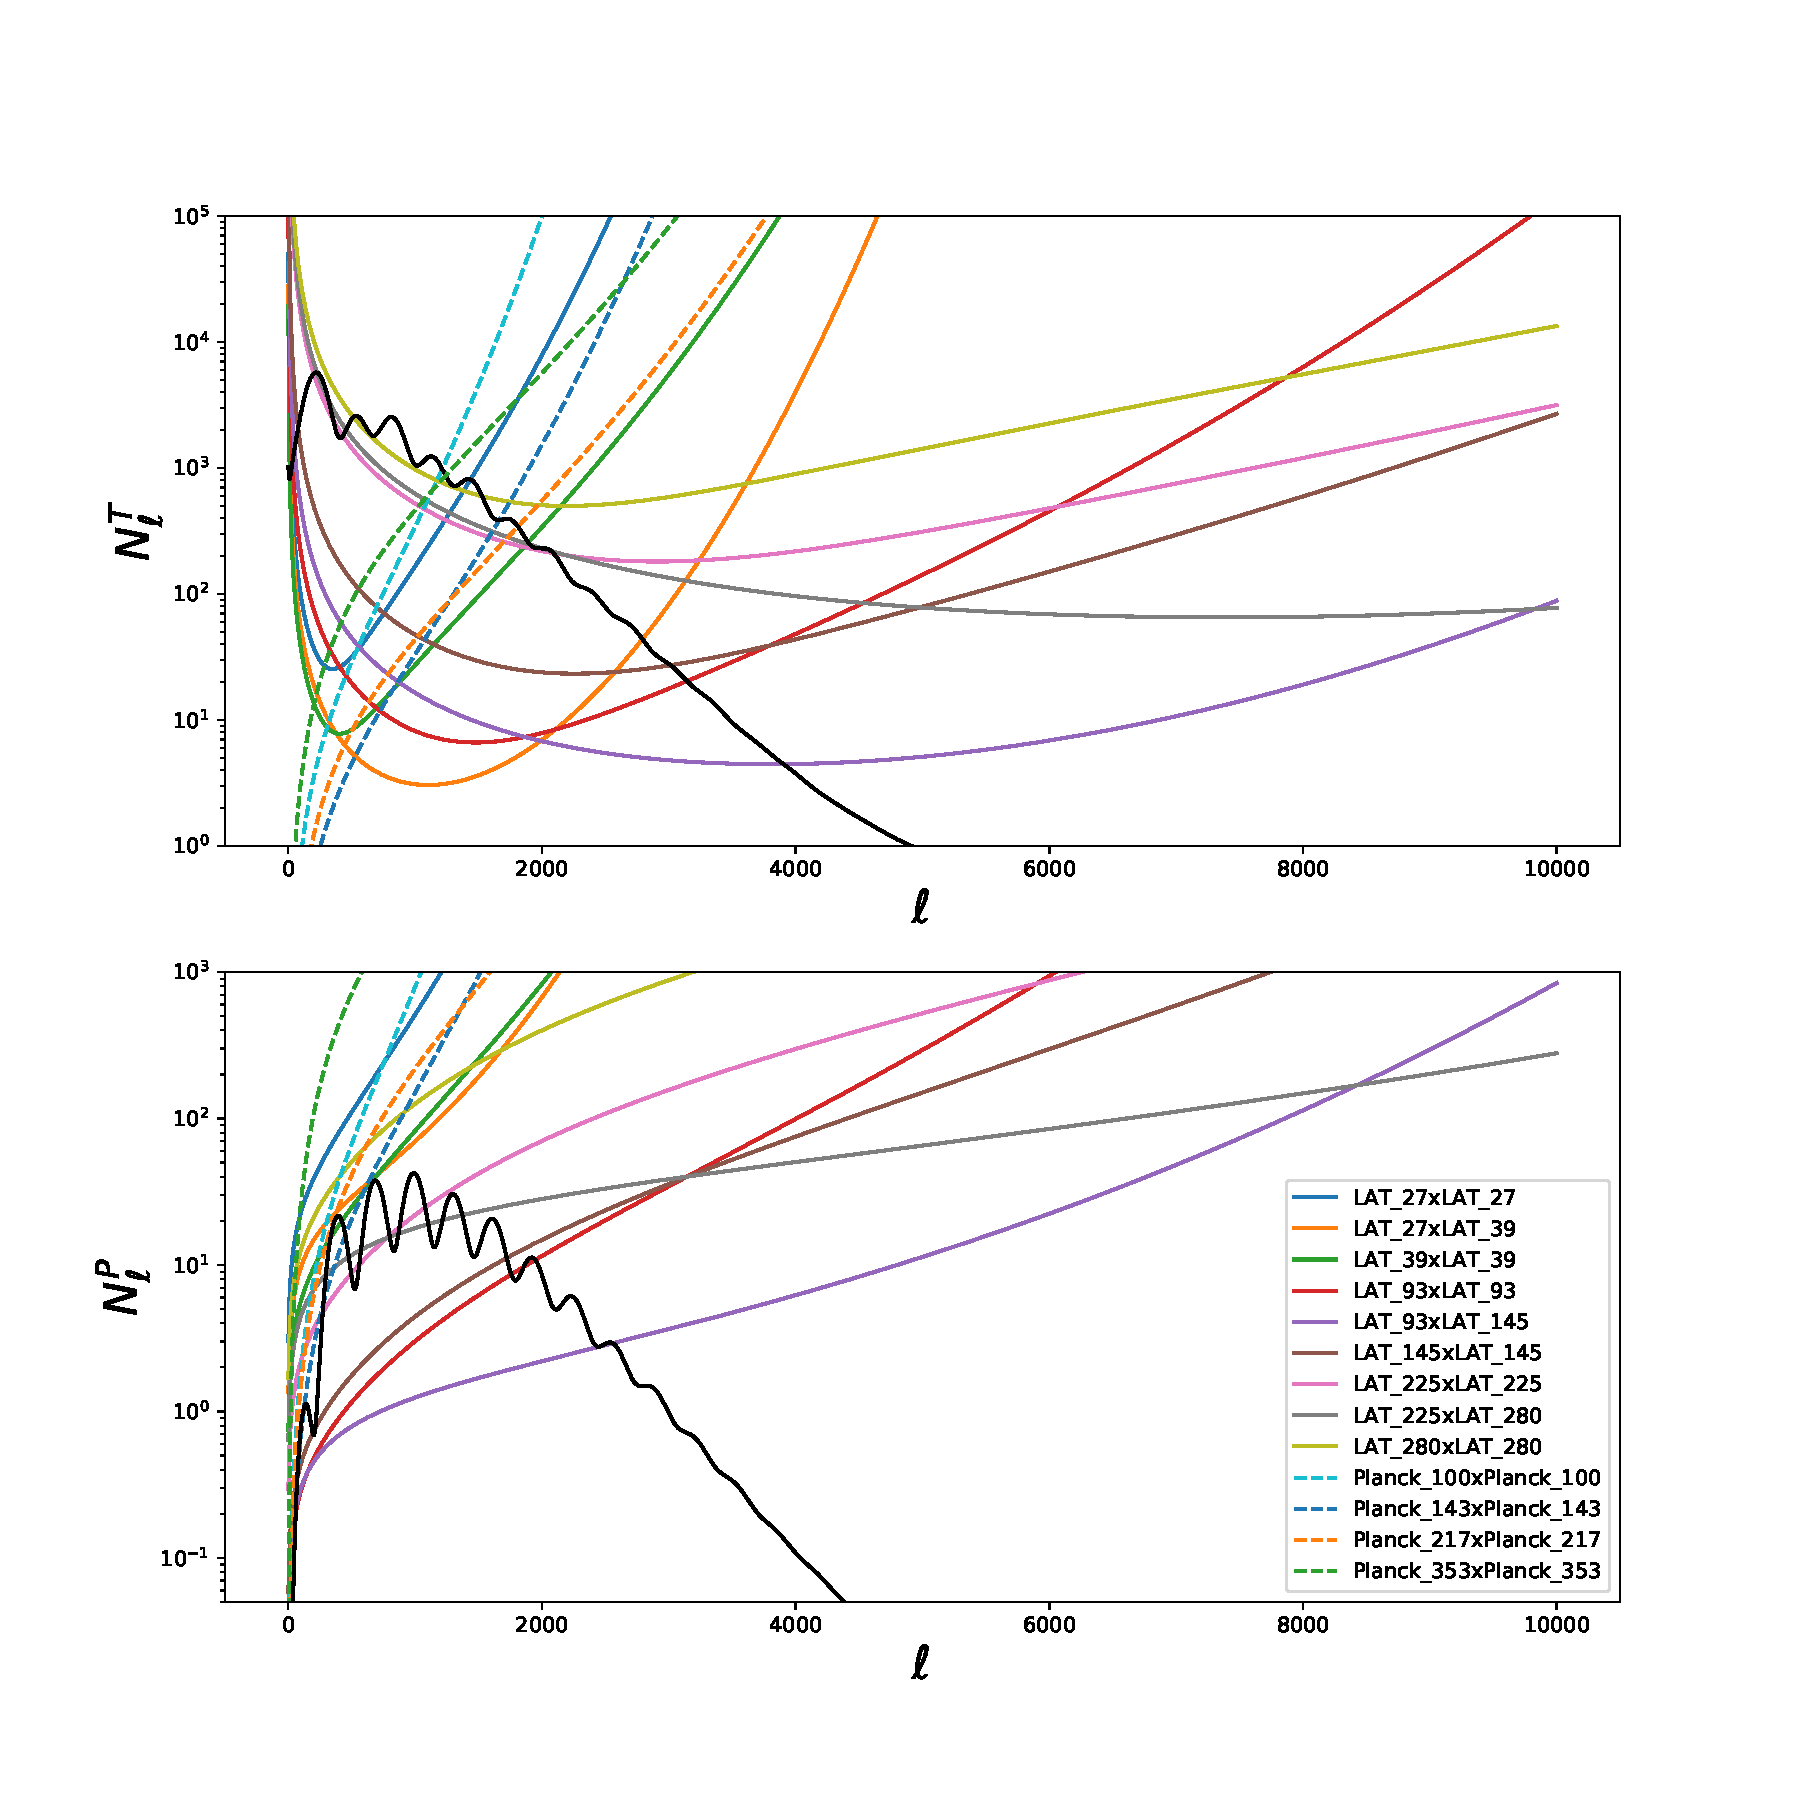
\includegraphics[width=1 \textwidth]{noise_ps_plot.pdf}
  \caption{Noise model for the the maps2params project.}
  \label{fig:noise_model}
\end{figure*}

\subsection{Data model}

We assume that the whole SO survey is mapped in two splits in time per frequency channel.
The data model for the k split at frequency $\nu$ in harmonic space is given by
\ba
a^{T, k}_{\ell m, \nu} &=&  b_{\ell, \nu} (a^{\rm T_{CMB}}_{\ell m} + a^{\rm fg}_{\ell m, \nu}) + n^{k}_{\ell m, \nu}  \\
a^{E, k}_{\ell m, \nu} &=&  b_{\ell, \nu} a^{\rm E_{CMB}}_{\ell m}  + n^{k}_{\ell m, \nu} \\
a^{B, k}_{\ell m, \nu} &=&  b_{\ell, \nu} a^{\rm B_{CMB}}_{\ell m}  + n^{k}_{\ell m, \nu}
\ea
Which in real space become a set of maps
\ba
T^{k}_{\nu}(\hat{n}) &=&  \sum_{\ell m }  a^{T, i}_{\ell m, \nu} Y_{\ell m} \\
Q^{k}_{\nu}(\hat{n}) \pm i U^{k}_{\nu}(\hat{n})  &=&  - \sum_{\ell m} (a^{E}_{\ell m, \nu} \pm i a^{B}_{\ell m, \nu}) {}_{\pm 2} Y_{\ell m} (\hat{n})
\ea
Since SO will have access to only part of the sky, we also include a mask $W^{\nu}(\hat{n})$ and we denote the observed temperature and polarisation field by
\ba
\tilde{T}^{k}_{\nu}(\hat{n}) &=&  W_{\nu}(\hat{n}) T^{k}_{\nu}(\hat{n}) \\
\tilde{Q}^{k}_{\nu}(\hat{n}) \pm i \tilde{U}^{k}_{\nu}(\hat{n}) &=& W_{\nu}(\hat{n}) (Q^{k}_{\nu}(\hat{n}) \pm i U^{k}_{\nu}(\hat{n}))  
\ea
An example of a SO mask in equatorial coordinate, including galactic mask and survey mask is presented in Figure \ref{fig:mask}. 
 
\begin{figure*}
  \centering
  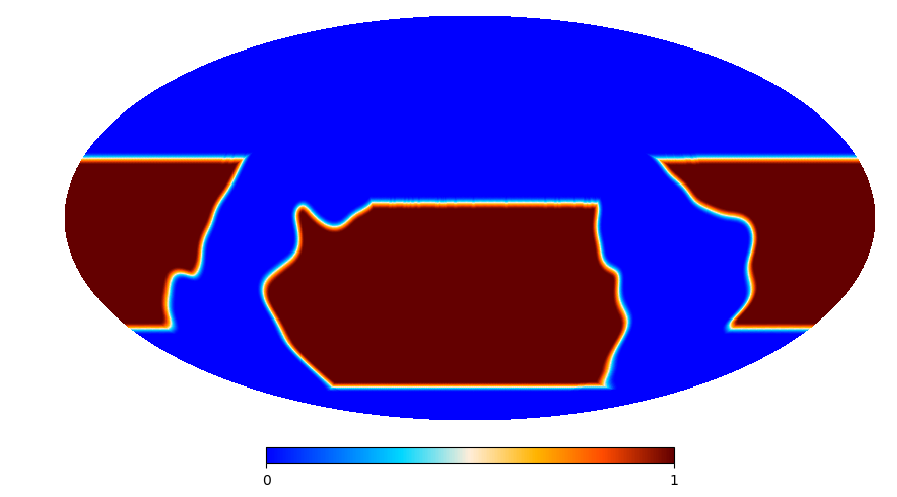
\includegraphics[width=1 \textwidth]{window_LAT_145.png}
  \caption{SO mask in equatorial coordinate, including galactic mask and survey mask.}
  \label{fig:mask}
\end{figure*}




\section{Computation of spectra}

\subsection{Power spectra estimator}

The binned pseudo cross power spectrum between the split i,j of the fields X and Y ($X, Y \in \{T,E,B \}$) at frequency $\nu_{1}$ and $\nu_{2}$ can be written
\ba
\tilde{D}^{X_{\nu_{1}}Y_{\nu_{2}}}_{b, ij} &=& \sum_{\ell} P^{(D_{\ell})}_{b \ell} \tilde{C}^{X_{\nu_{1}}Y_{\nu_{2}}}_{\ell, ij} \\
\tilde{C}^{X_{\nu_{1}}Y_{\nu_{2}}}_{\ell, ij}  &=&  \frac{1}{2\ell +1} \sum_{m}  a^{X, i}_{\ell m, \nu_{1}}  a^{Y, j, *}_{\ell m, \nu_{2}}
\ea
\ba
P^{(D_{\ell})}_{b \ell} &=&.  \frac{\ell (\ell+1) }{ 2\pi \Delta \ell_{b}} \ \ \ell^{\rm low}_{b} \le \ell \le \ell^{\rm high}_{b} \nonumber \\
&=& 0 \ \ {\rm otherwise}
\ea
 
To go from pseudo power spectrum estimator to unbiased estimate we compute the mode coupling matrix

\tiny
\ba
 \begin{pmatrix} \langle \tilde{D}^{T_{\nu_{1}}T_{\nu_{2}}}_{b} \rangle  \cr \langle \tilde{D}^{T_{\nu_{1}}E_{\nu_{2}}}_{b} \rangle  \cr \langle \tilde{D}^{T_{\nu_{1}}B_{\nu_{2}}}_{b} \rangle  \cr \langle \tilde{D}^{E_{\nu_{1}}T_{\nu_{2}}}_{b} \rangle  \cr \langle \tilde{D}^{B_{\nu_{1}}T_{\nu_{2}}}_{b} \rangle  \cr \langle \tilde{D}^{E_{\nu_{1}}E_{\nu_{2}}}_{b} \rangle  \cr \langle \tilde{D}^{E_{\nu_{1}}B_{\nu_{2}}}_{b} \rangle \cr  \langle \tilde{D}^{B_{\nu_{1}}E_{\nu_{2}}}_{b} \rangle \cr \langle \tilde{D}^{B_{\nu_{1}}B_{\nu_{2}}}_{b} \rangle \end{pmatrix} = \sum_{\ell_{1}}
\begin{pmatrix} 
M^{\nu_{1}\nu_{2}00}_{bb_{1}} & 0 &0 &0 &0 &0 &0 &0 &0 &
\cr
0 & M^{\nu_{1}\nu_{2}02}_{bb_{1}} & 0 &0 &0 &0 &0 &0 &0 &
\cr
0 &0 & M^{\nu_{1}\nu_{2}02}_{bb_{1}} &0 &0 &0 &0 &0 &0 &
\cr
0 &0 & 0 & M^{\nu_{1}\nu_{2}02}_{bb_{1}} &0 &0 &0 &0 &0 &
\cr
0 &0 & 0 &0 & M^{\nu_{1}\nu_{2}02}_{bb_{1}} &0 &0 &0 &0 &
\cr
0 &0 &0 &0 &0 & M^{\nu_{1}\nu_{2}++}_{bb_{1}} & 0 &0 & M^{\nu_{1}\nu_{2}--}_{bb_{1}} &
\cr
0 &0 &0 &0 &0 &0 & M^{\nu_{1}\nu_{2}++}_{bb_{1}} &-M^{\nu_{1}\nu_{2}--}_{bb_{1}} & 0 &
\cr
0 & 0 & 0 & 0 & 0 & 0&  -M^{\nu_{1}\nu_{2}--}_{bb_{1}}  & M^{\nu_{1}\nu_{2}++}_{bb_{1}}  & 0&
\cr
0 & 0 & 0 & 0 & 0 & M^{\nu_{1}\nu_{2}--}_{bb_{1}} &  0 & 0 & M^{\nu_{1}\nu_{2}++}_{b_{1}} &
\end{pmatrix}
\begin{pmatrix} \langle D^{T_{\nu_{1}}T_{\nu_{2}}}_{b_{1}} \rangle  \cr \langle D^{T_{\nu_{1}}E_{\nu_{2}}}_{b_{1}} \rangle  \cr \langle D^{T_{\nu_{1}}B_{\nu_{2}}}_{b_{1}} \rangle  \cr \langle D^{E_{\nu_{1}}T_{\nu_{2}}}_{b_{1}} \rangle  \cr \langle D^{B_{\nu_{1}}T_{\nu_{2}}}_{b_{1}} \rangle  \cr \langle D^{E_{\nu_{1}}E_{\nu_{2}}}_{b_{1}} \rangle  \cr \langle D^{E_{\nu_{1}}B_{\nu_{2}}}_{b_{1}} \rangle \cr  \langle D^{B_{\nu_{1}}E_{\nu_{2}}}_{b_{1}} \rangle \cr \langle D^{B_{\nu_{1}}B_{\nu_{2}}}_{b_{1}} \rangle \end{pmatrix}\ea
\normalsize
\ba
M^{\nu_{1}\nu_{2}XY}_{bb_{1}} &=& \sum_{\ell \ell_{1}} P^{(D_{\ell})}_{b \ell} M^{\nu_{1}\nu_{2}XY}_{\ell \ell_{1}} B^{\nu_{1}}_{\ell_{1}}B^{\nu_{2}}_{\ell_{1}}  Q^{(D_{\ell})}_{\ell_{1}b_{1}} \\
Q^{(D_{\ell})}_{\ell b} &=& \frac{2\pi}{\ell (\ell+1)}  \ \ \ell^{\rm low}_{b} \le \ell \le \ell^{\rm high}_{b} \nonumber \\
&=& 0 \ \ {\rm otherwise} \nonumber \\
\ea
$B^{\nu}_{\ell}$ is the harmonic transform of the beam at frequency $\nu$.
A detailed computation of the different mode coupling elements is given in the pspy doc. We remind the expression of the elements below
\ba
M^{\nu_{1}\nu_{2}00}_{ \ell, \ell_1} &=&   \frac{2\ell_1 +1}{4\pi}  \sum_{ \ell_3} (2\ell_3+1) {\cal W}^{\nu_{1}\nu_{2}}_{\ell_3} 
\left(\begin{array}{clcr}
\ell & \ell_1 & \ell_3\\
0 & 0 & 0 \end{array}\right)^{2} \nonumber \\
M^{\nu_{1}\nu_{2}++}_{\ell \ell_{1}} &=& \frac{2\ell_1 +1}{4\pi}  \sum_{\ell_{3}} (2\ell_3 +1) {\cal W}^{\nu_{1}\nu_{2}}_{\ell_3} \left(\begin{array}{clcr}
\ell & \ell_1 & \ell_3\\
2 & -2 & 0 \end{array}\right)^{2} \frac{(1+ (-1)^{\ell + \ell_1 + \ell_3})}{2} \nonumber \\
M^{\nu_{1}\nu_{2}--}_{\ell \ell_{1}} &=& \frac{2\ell_1 +1}{4\pi}  \sum_{\ell_{3}} (2\ell_3 +1) {\cal W}^{\nu_{1}\nu_{2}}_{\ell_3} \left(\begin{array}{clcr}
\ell & \ell_1 & \ell_3\\
2 & -2 & 0 \end{array}\right)^{2} \frac{(1- (-1)^{\ell + \ell_1 + \ell_3})}{2} \nonumber \\
M^{\nu_{1}\nu_{2}02}_{\ell \ell_{1}} &=& \frac{2\ell_1 +1}{4\pi}  \sum_{\ell_{3}} (2\ell_3 +1) {\cal W}^{\nu_{1}\nu_{2}}_{\ell_3} \left(\begin{array}{clcr}
\ell & \ell_1 & \ell_3\\
2 & -2 & 0 \end{array}\right) 
\left(\begin{array}{clcr}
\ell & \ell_1 & \ell_3\\
0 & 0 & 0 \end{array}\right)
\ea
An unbiased estimate of the binned cross power spectrum between the split i,j of the fields X and Y ($X, Y \in \{T,E,B \}$) at frequency $\nu_{1}$ and $\nu_{2}$ is finally obtained
\ba
\hat{D}_{b, ij}^{X_{\nu_{1}}Y_{\nu_{2}}}= (\bm{M}^{-1})^{X_{\nu_{1}}Y_{\nu_{2}}W_{\nu_{1}}Z_{\nu_{2}}}_{bb_{1}} \tilde{D}_{b_{1}, ij}^{W_{\nu_{1}}Z_{\nu_{2}}}
\ea

\subsection{Combinatorics}

We will consider two different types of spectra. The auto power spectra, they have non zero noise bias, and the cross power spectrum free from noise bias
\ba
\hat{D}^{\rm auto, X_{\nu_{1}}Y_{\nu_{2}}}_{b} = \sum_{ij}  \hat{D}^{X_{\nu_{1}}Y_{\nu_{2}}}_{b, ij} \delta_{ij} \\
\hat{D}^{\rm cross, X_{\nu_{1}}Y_{\nu_{2}}}_{b} = \sum_{ij}  \hat{D}^{X_{\nu_{1}}Y_{\nu_{2}}}_{b, ij} (1- \delta_{ij})
\ea
Note that if we consider that different frequency channel have independent noise, the expression become
\ba
\hat{D}^{\rm auto, X_{\nu_{1}}Y_{\nu_{2}}}_{b} = \sum_{ij}  \hat{D}^{X_{\nu_{1}}Y_{\nu_{2}}}_{b, ij} \delta_{ij} \delta_{\nu_{1} \nu_{2}}\\
\hat{D}^{\rm cross, X_{\nu_{1}}Y_{\nu_{2}}}_{b} = \sum_{ij}  \hat{D}^{X_{\nu_{1}}Y_{\nu_{2}}}_{b, ij} (1- \delta_{ij} \delta_{\nu_{1} \nu_{2}})
\ea
This will not be the case for SO, because dichroic arrays see the same atmospheric noise.


\section{Computation of analytic covariance matrices}




We estimate analytically the different covariance elements for the TT, TE and EE power spectrum as

\ba
\langle \Delta \tilde{C}^{R_{\nu_{1} \alpha}S_{\nu_{2} \beta}}_{\ell_{1}} \Delta  \tilde{C}^{X_{\nu_{3} \gamma}Y_{\nu_{4} \eta}}_{\ell_{2}}\rangle &=&      \chi_{RX,SY,\ell_{1}\ell_{2}}^{\nu_{1} \alpha \times \nu_{3} \gamma, \nu_{2} \beta \times  \nu_{4} \eta} M^{00}_{\ell_{1} \ell_{2}}(W_{R}^{\nu_{1}, } W_{X}^{\nu_{3}},W_{S}^{ \nu_{2} }W_{Y}^{ \nu_{4} })\nonumber \\
& +&  \chi_{RY,SX,\ell_{1}\ell_{2}}^{\nu_{1} \alpha \times \nu_{4} \beta, \nu_{2} \beta \times  \nu_{3} \gamma}  M^{00}_{\ell_{1} \ell_{2}}(W_{R}^{\nu_{1}}W_{Y}^{ \nu_{4} },W_{S}^{ \nu_{2} }W_{X}^{\nu_{3}})
\ea


With 
\ba
 \chi_{RX,SY}^{\nu_{1} \alpha \times \nu_{3} \gamma, \nu_{2} \beta \times  \nu_{4} \eta} &=&  C^{\nu_{1} \alpha \times \nu_{3} \gamma}_{RX, \ell}   C^{ \nu_{2} \beta \times  \nu_{4} \eta}_{SY, \ell} +  C^{\nu_{1} \alpha \times \nu_{3} \gamma}_{RX, \ell}  \tilde{N}^{ \nu_{2} \beta \times  \nu_{4} \eta}_{SY, \ell}  f^{\alpha \gamma}_{\beta \eta} + C^{ \nu_{2} \beta \times  \nu_{4} \eta}_{SY, \ell} \tilde{N}^{\nu_{1} \alpha \times \nu_{3} \gamma}_{RX, \ell}   f^{\beta \eta}_{\alpha \gamma} \nonumber \\ & +&  g_{\alpha \gamma, \beta \eta} \tilde{N}^{\nu_{1} \alpha \times  \nu_{3} \gamma}_{RX, \ell}\tilde{N}^{ \nu_{2} \beta \times  \nu_{4} \eta}_{SY, \ell} \nonumber \\
g_{\alpha \gamma, \beta \eta} &=& \frac{n^{2}_{s} \delta_{\alpha \gamma}\delta_{\beta \eta} -n_{s} \delta_{\alpha \beta \gamma \eta}}{n^{2}_{s}(n_{s} -\delta_{\alpha \beta}) (n_{s} -\delta_{\gamma \eta})} \nonumber \\
 f^{\beta \eta}_{\alpha \gamma}  &=& \frac{n^{3}_{s}\delta_{\alpha \gamma}- n^{2}_{s}( \delta_{\alpha \beta \gamma} + \delta_{\alpha  \gamma \eta}) + n_{s} \delta_{\alpha \beta \gamma \eta}}{n^{2}_{s}(n_{s} -\delta_{\alpha \beta}) (n_{s} -\delta_{\gamma \eta})} \nonumber\\
\ea

$n_{s}$ is the number of splits of data and $\tilde{N}^{ \nu_{2} \beta \times  \nu_{4} \eta}_{SY, \ell}$ is the effective noise spectrum $ \tilde{N}^{ \nu_{2} \beta \times  \nu_{4} \eta}_{SY, \ell} = \frac{N^{ \nu_{2} \beta \times  \nu_{4} \eta}_{SY, \ell}}{ b_{\ell}^{\nu_{2}, \beta} b_{\ell}^{\nu_{3}, \eta} }$

An example of a full analytic covariance matrix for three frequencies of LAT data is shown in Figure \ref{fig:cov}.

\begin{figure*}
  \centering
  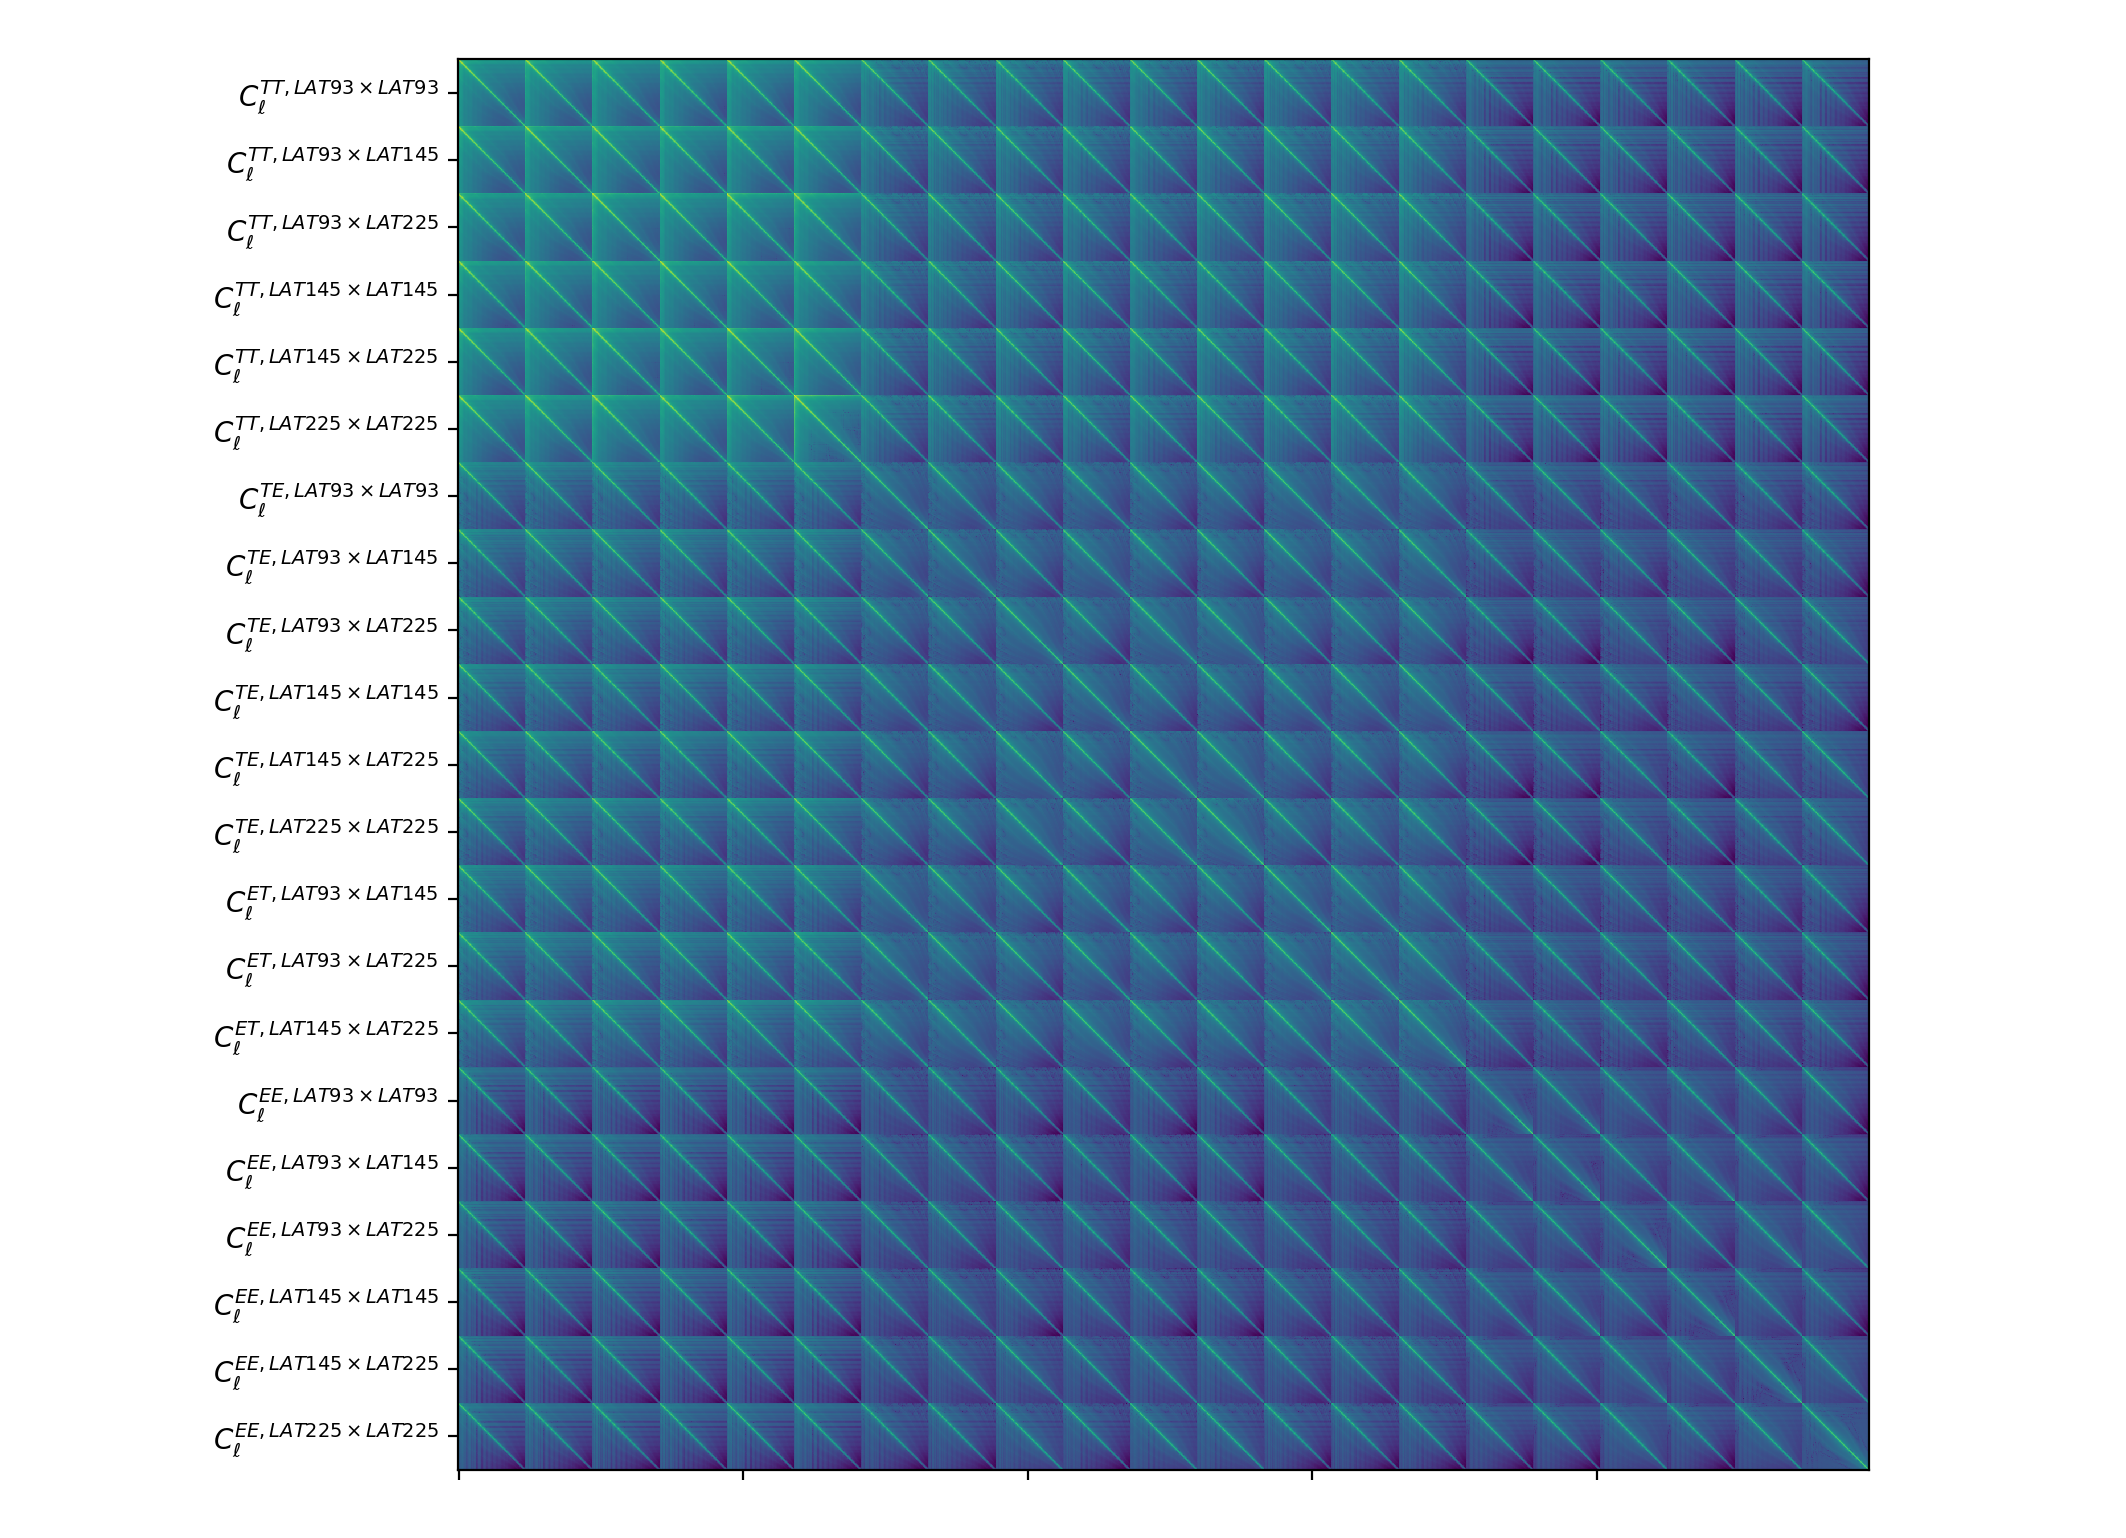
\includegraphics[width=1 \textwidth]{covariance.png}
  \caption{Covariance matrix for three frequency channels of LAT data.}
  \label{fig:cov}
\end{figure*}



\end{document}
